Here, we describe a numerical measure of sound level (or amplitude), which aims to predict (or at least correlate with) perceived loudness.

%% Audible Energy
\subsection{Mean audible energy (\texorpdfstring{$\lambda$}{lambda})}\label{sec:04_Auditory_Models:Audible_Energy}
We define the \textit{mean audible energy} (MAE), $\lambda$, of an ambisonics signal as the average energy of the zeroth-order term across a set of critical bands,%
\footnote{Roughly speaking, a \textit{critical band} refers to the bandwidth of the effective auditory filter created by the cochlea, within which a stronger second tone will mask the perception of a weaker first tone \citep[chapter 3]{Moore2013}.}
 i.e.,
\begin{equation}\label{eq:04_Auditory_Models:Mean_Audible_Energy}
\lambda = 10 \log_{10} \left( \frac{1}{N_b} \sum_{c = 1}^{N_b} \frac{\displaystyle \int_{-\infty}^\infty |H_\Gamma(f;f_c)| |A_0(f)|^2 df}{\displaystyle \int_{-\infty}^\infty |H_\Gamma(f;f_c)| df} \right),
\end{equation}
where $|\cdot|$ again denotes the absolute value of the argument and $H_\Gamma(f;f_c)$ is the transfer function of a gammatone filter%
\footnote{In this work, we used the gammatone filters implemented in the large time-frequency analysis toolbox (LTFAT) for MATLAB \citep{LTFATURL}.} (which approximates critical bands) with center frequency $f_c$ for $c \in [1, N_b]$, for a set of ERB-spaced (equivalent rectangular bandwidth) center frequencies \citep{GlasbergMoore1990} spanning the range $f \in [50~\text{Hz}, 21~\text{kHz}]$.
Magnitude responses of the first four of these filters are shown in \figref{fig:04_Auditory_Models:Gammatone_Filters}.
As shown in that plot, these filters effectively act as narrow band-pass filters, and the spacing between adjacent filters decreases with increasing frequency (when plotted on a logarithmic axis) due to the ERB spacing.
Due to these filters, the summand in \eqnref{eq:04_Auditory_Models:Mean_Audible_Energy} approximately represents the power spectrum of a signal reaching the cochlea, as defined by \citet[Eq.~(5.12)]{Salomons1995PhD}.

\begin{figure*}[t]
    	\centering
    	\begin{subfigure}[b]{0.49\textwidth}
        		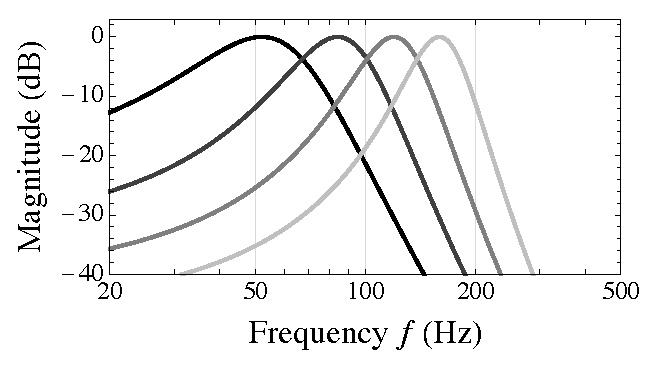
\includegraphics[width=\textwidth]{04_auditory_models/figures/gammatone_mag.eps}
        		\caption{Gammatone filters, $H_\Gamma$}
        		\label{fig:04_Auditory_Models:Gammatone_Filters}
    	\end{subfigure}
	\hfill
    	\begin{subfigure}[b]{0.49\textwidth}
        		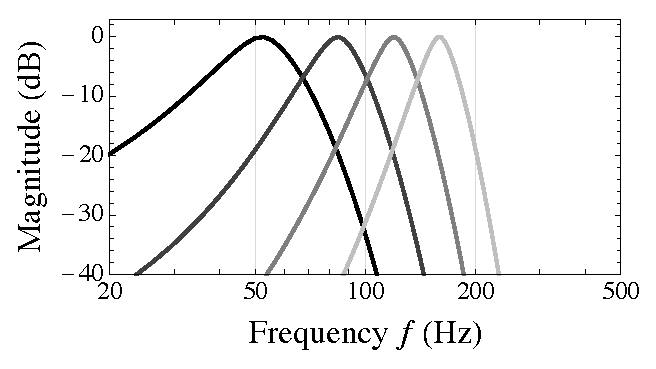
\includegraphics[width=\textwidth]{04_auditory_models/figures/patterson_mag.eps}
        		\caption{Patterson's filters, $H_\text{P}$}
        		\label{fig:04_Auditory_Models:Patterson_Filters}
    	\end{subfigure}
	
	\caption[Magnitude responses of gammatone filters and Patterson's filters.]{
	Magnitude responses of gammatone filters (left panel) and Patterson's filters (right) for the first four ERB-spaced center frequencies increasing from approximately 50~Hz.}
	\label{fig:04_Auditory_Models:Auditory_Filters}
\end{figure*}

We further define the level error given in dB by
\begin{equation}\label{eq:04_Auditory_Models:Audible_Energy_Difference}
e_\lambda = \tilde{\lambda} - \lambda,
\end{equation}
where $\lambda$ is the MAE for a reference signal and $\tilde{\lambda}$ is that for a test signal.